\chapter{Competitor Rules}

\section{Safety}

Riders must wear shoes, knee pads and gloves (definitions in chapter \ref{chap:general_definitions}).

Helmets are required for Downhill Gliding.
Riders on wheels larger than 24 Class (or with gearing) must also wear helmets.

\section{Unicycles}

Only regular unicycles may be used.
Riders may use different unicycles for different racing events, as long as all comply with the rules for events in which they are entered.

For events divided by wheel size, there is a allowable tire diameter range and minimum crank arm length for each Unicycle Class:

\begin{longtable}{|p{2.8cm}|p{4.6cm}|p{3.6cm}|p{2.5cm}|}
\hline
\textbf{Unicycle Class} & \textbf{Diameter Range} & \textbf{Min Crank Length} & \textbf{Transmission}\\
\hline
16 Class & 0 -- 418mm & 89mm & regular \\
\hline
20 Class & more than 418mm -- 518mm & 100mm & regular \\
\hline
24 Class & more than 518mm -- 618mm & 125mm & regular \\
\hline
29 Class & more than 618mm -- 778mm & No limit & regular \\
\hline
Unlimited Class & No limit & No limit & unlimited \\
\hline
\end{longtable}

Any unicycles in question must be checked for compliance within their wheel class (wheel diameter, crank length and transmission), with the tire pressure that will be used in the race.
Preferably, this check is carried out immediately before the race.

Crank arm length is measured from the center of the wheel axle to the center of the pedal axle.
Longer sizes may be used.

In all track racing events on regular unicycles, shoes must not be fixed to the pedals in any way (no click-in pedals, toe clips, tape, magnets or similar).

\section{Rider Identification}

Riders must wear their race number clearly visible on their chest so that it is visible during the event and as the rider crosses the finish line (as relevant).
Additionally, the rider may be required to wear a chip for electronic timing.

\section{Protests}

Protests must be filed on an official form.
Mistakes in paperwork, inaccuracies in placing, and interference from other riders or other sources are all grounds for protests.
All Referee decisions are final, and cannot be protested.
For a large event such as Unicon or continental championships, the default protest time is 60 minutes (counting from the posting of results), the minimum is 30 minutes.
For smaller events, the default protest time is 30 minutes, the minimum is 15 minutes.
Every deviation from the default protest time has to be clearly announced when the results are posted, including stating the protest deadline on the results list itself.
The protest time may be extended for riders who have to be in other races during the protest period.
All protests will be acknowledged within 30 minutes from the time they are received, and an effort will be made to settle the issue within those 30 minutes.

\section{Wheel Size Categories}

Wheel sizes for track racing are 20 Class, 24 Class and 29 Class.
Additional groups for 16 Class or other wheels can be added.
When not otherwise specified, 24 Class is the maximum wheel size above age 10.
For age groups with a maximum age of 10 or younger, the maximum wheel size is 20 Class (or smaller, if smaller sizes are also used).

The youngest age group for 24 Class wheels should have a minimum age of 0, so riders 10 and younger have the option of racing on 24 Class with those groups (e.g. 0-8 on 20 Class, 9-10 on 20 Class, 0-13 on 24 Class).

Unless otherwise specified, it is allowed to ride in any particular Class with a unicycle that fully conforms to a smaller Class
(e.g.\ a 20 Class unicycle is allowed in a 24 Class race).

\section{Racing Disciplines}

\subsection{100m Race}

In the 100m race, riders must stay in their lane.

\subsection{400m Race}

The 400m race is started with a stagger start, where riders are started in separate lanes, at separate locations.
In the 400m race, riders must stay in their lane.

\subsection{800m Race}

There are two different ways to run an 800m race, remounting after a dismount is allowed in both ways:

\textbf{1. 800m Race with Stagger Start:} Riders are started in separate lanes, at separate locations.
The race shall be run in lanes as far as the nearer edge of the breakline where riders may leave their respective lanes.
The breakline shall be an arced line marked after the first bend across all lanes other than lane 1.
To assist athletes identify the breakline, halved tennis balls can be placed on the lane lines immediately before the intersection of the lines and the breakline.
After the breakline, non-lane racing rules apply (see section \ref{subsec:track_lane-use_non-lane-races}).

\textbf{2. 800m with Waterfall Start:} Riders are started at a curved starting line that places all riders an equal distance from the first turn.
If a waterfall start is used, non-lane rules apply from the start.

\subsection{One Foot Race}
The distance of the One Foot Race is 50m.
Riders may pedal with both feet for the first 5 meters, but must be pedaling with only one foot after crossing the 5m line.
The non-pedaling foot must have left the pedal when the tire contact point crosses the 5m line on the track.
The non-pedaling foot may or may not be braced against the unicycle fork.

\subsection{Wheel Walk Race}

Riders start mounted, with one or both feet on the tire, and propel the unicycle only by pushing the tire with one or both feet.
No contact with pedals or crank arms is allowed.
No crank arm restrictions.
Riders in age groups with a maximum age of 10 or younger will race a 10m Wheel Walk.
All other riders will race a 30m Wheel Walk.

\subsection{Relay (Track)}
The relay distances shall be 4 x 100m or 4 x 400m like in athletics

In the 4 x 100m relay each takeover zone shall be 30m long, in the 4 x 400m relay each takeover zone shall be 20m.
The takeover zones must be marked on the track.
(The zones shall start and finish at the edges of the zone lines nearest the start line in the running direction.)
In the 4 x 100m relay, riders are not permitted to line up outside their takeover zones, and shall start within the zone.
In the 4 x 400m relay, there is no defined preparation area for the next riders as long as they stay within their lanes.
Riders may remount if necessary, and must pick up the baton if it is dropped.
The handover of the baton must be within the takeover zone.
This means that before the baton crosses the start mark of the takeover zone only the incoming rider is in touch with the baton and at the end of the takeover zone only the outgoing rider is in touch with the baton.
Riders may not throw the baton to make a pass and may not touch the ground with any part of their body while making a pass.
If the baton is not handed over within the marked takeover zone, the team will be disqualified.
Leaving of the lane within the takeover zone or when remounting does not result in disqualification as long as the riders do not obstruct, impede or interfere with another rider’s progress.

Mixed male/female teams may be used, and reasonable age groups may be used depending on the number of expected competitors of the event.
Each relay team may have any mix of ages, the age of the oldest rider determines the age group.

\subsection{Other Wheel Size Races}
The host can choose to offer additional track events based upon other wheel size requirements.
Two examples include 700c racing and Unlimited.
Exclusive of unicycle requirements, all other track racing rules apply.

An unlimited race is one in which there are no unicycle size restrictions.
Any size wheels, any length crank arms, giraffes or any types of unicycles (see definition in chapter \ref{chap:general_definitions}) are allowed.

In the 700c wheel category, unicycle wheels must be greater than 618mm in diameter, have a maximum bead seat diameter (BSD) of 622 mm, and there are no restrictions on crank length.

\section{Racing Rules}

\subsection{Riders Must Be Ready}

Riders must be ready when called for their races.
Riders not at the start line when their race begins may lose their chance to participate.
The Starter will decide when to stop waiting, remembering to consider language barriers, and the fact that some riders may be slow because they are helping run the convention.

\subsection{Starting \label{subsec:track_starting}}

This procedure is used for all Track Races, unless noted otherwise.

Riders start mounted, holding onto a starting post or other support.

Usually, a start-beep apparatus is used.
This provides a six-count start: ``beep - beep -beep - beep - beep - buup!''
The timing between (the start of) successive beeps is one second.
The first five beeps have all the same sound frequency.
The final tone (buup) has a higher frequency, so that the competitors can easily distinguish this tone from the rest. The proper moment to start is the beginning of the final tone.

As an alternative, the Starter will give a three-count start before firing a starting gun on the fourth count.
Example: ``One, two, three, BANG!''
The time between each of these elements should be the same, and approximately 3/4 seconds.
This allows riders to predict the timing of the gun, for a fair start.

Riders start with the fronts of their tires (forward most part of wheel) behind the edge of the starting line that is farthest from the finish line.
Rolling starts are not permitted in any race.
Riders may start from behind the starting line if they wish, provided all other starting rules are followed.
Riders may lean before the start, but their wheels may not move forward during the start beeps or counting down.
Rolling back is allowed.
Riders may place starting posts in the location most comfortable for them, as long as it doesn't interfere with other riders.

\subsection{False Starts \label{subsec:track_false-starts}}

A false start occurs if a rider's wheel moves forward before the start signal, or if one or more riders are forced to dismount due to interference from another rider or other source.

If a heat has to be restarted, the Starter will immediately recall the riders, for example by blowing a whistle or other clear and predefined signal.
Only the earliest false starting rider gets assigned this false start and the associated warning or disqualification.

There are two options on how to deal with false starts:
\begin{itemize}

\item \textbf{One False Start Allowed Per Heat:}
After the first false start of a particular heat, all riders may start again.
Thereafter, any rider(s) causing a false start are disqualified for this event.
This option should not be used without an electronic false start monitoring system.
\item \textbf{One False Start Allowed Per Rider:}
After the first false start of a particular rider in a heat, the rider in question receives a warning and may start again.
Any rider(s) causing their personal second false start are disqualified.
\end{itemize}

\subsection{Lane Use}

In most races, a rider must stay in his or her own lane, except when the rider has to swerve to avoid being involved in a crash.
In all other cases, a rider who goes outside their lane is disqualified.
Going outside a track lane means that the tire of the unicycle touches the ground outside his assigned lane.
Riding on the marking is allowed.
No physical contact between riders is allowed during racing.

\subsection{Passing in Non-Lane Races \label{subsec:track_lane-use_non-lane-races}}

This applies to 800m and other events without lanes.
No physical contact between riders is allowed.
In track races, an overtaking rider must pass on the outside, unless there is enough room to safely pass on the inside.
Riders passing on the inside are responsible for any fouls that may take place as a result.
Riders must maintain a minimum of one (24 Class) wheel diameter (618 mm as judged by eye) between each other when passing, and at all other times.
This is measured from wheel to wheel, so that one rider passing another may come quite close, as long as their wheels remain at least 618 mm apart.
The slower rider must maintain a reasonably straight course, and not interfere with the faster rider.

\subsection{Dismounts}

A dismount is any time a rider's foot or other body part touches the ground.
Except for the 800m, Relay races, and other races where this is announced in advance, after a dismount the race may not be continued and will be considered as not finished (DNF - Did Not Finish).
In races where riders are allowed to remount and continue, riders must immediately remount at the point where the unicycle comes to rest, without running.
If a dismount puts the rider past the finish line, the rider must back up and ride across the line in control, in the normal direction.

\subsection{Assisting Racers}

In races where riders are allowed to remount, the riders must mount the unicycle completely unassisted.
Spectators or helpers may help the rider to his or her feet and/or retrieve the dropped unicycle, but the rider (and the unicycle) may not have any physical contact with any outside object or person, including a starting block under the wheel, when mounting.

\subsection{Illegal Riding}

This includes intentionally interfering in any way with another rider, deliberately crossing in front of another rider to prevent him or her from moving on, deliberately blocking another rider from passing, or distracting another rider with the intention of causing a dismount.
A rider who is forced to dismount due to interference by another rider may file a protest immediately at the end of the race.
Riders who intentionally interfere with other riders may receive from the Referee a warning, a loss of placement (given the next lower finishing place), disqualification from that race/event, or suspension from all races.

\subsection{Second Attempt After Hindrance or Interference}

If a rider is hindered due to the actions of another rider, or outside interference, either during the start or during the race, he or she may request to make a second attempt.
The Referee decides if the request is granted.
A second attempt must not be granted to a rider who is disqualified based on something that happened before they were hindered.

No complete definition of hindrance or interference can be given, but it does include cases where a rider swerves, hesitates and/or decelerates because this is arguably necessary in order to avoid a crash or potential crash.

If the request is granted, the Referee has two options:

\textbf{Option 1:}
Re-run the whole heat in question.\\
In general, this option is preferred only if the heat includes the fastest riders within an age group.
For the other riders in the heat, riding again is optional.
If they decide to ride again, they agree to discard their previous result.
If they don't ride again, their previous result stands.
If none of the other riders want to ride again, the Referee reverts to option 2.

\textbf{Option 2:}
Do any of (a), (b) or (c), depending on the conditions.\\
In general, this option is preferred if the heat in question did not include the fastest riders within an age group:
\begin{enumerate}[label=(\alph*)]
\item If possible, the rider is added to an upcoming heat in his own age group; or
\item If possible, the rider is added to an upcoming heat in another age group; or
\item If none of the above is possible, the rider does his second attempt in a dedicated heat.
\end{enumerate}
In option 2, the rider decides if he wants company or not.
He can pick the riders, but cannot hold up the proceedings to wait for them if other riders are available.
The Referee has the final say as to which extra riders are allowed to participate in such a heat.
It must be stated clearly to any accompanying riders that their result is not official.

In all cases, if the hindered rider is allowed to do a second attempt and decides to do so, the first run is canceled and only the second run counts regardless of the result.
In the case where a second attempt was incorrectly granted, for example when the rider was disqualified based on something that happened before the hindrance in question occurred, the result of the second attempt for that rider does not count and the result from the first run stands.

In non-lane races, if a rider is forced to dismount due to a fall by the rider immediately in front, it is considered part of the race -- not a reason to grant a second attempt -- and all riders involved may remount and continue.
The Referee can override this rule if intentional interference is observed.

\subsection{Finishes \label{sec:track_finishes}}

The finish moment is when the front of the tire crosses the finish.
The exact location of the finish is the edge of the finish line that is nearest to the starting line.
Riders are thus not timed by outstretched bodies.
At the finish moment, riders must be mounted and in control of the unicycle.
``Control'' is defined as follows:
\begin{enumerate}[label=(\alph*)]
\item in regular races: the rider has both feet on the pedals; or
\item in one-foot races: the rider has one foot on a pedal; or
\item in wheel walk races: the rider continues to wheel walk.
\end{enumerate}
In races where dismounting is allowed (800m, Relay, etc.\@), in the event that a rider does cross the finish line but not in control, the rider must back up on foot, remount and ride across the finish line in control.
In races where dismounting is not allowed, the rider is disqualified.

\subsection{Finals}

At Unicons, a `final' must be held for each of the following races: 100m, 400m, 800m, One Foot, Wheel Walk, and IUF Slalom.
For any other Track discipline, a `final' may be held at the discretion of the organizer, after all age group competition for that discipline has been completed.

For disciplines that are run in heats, such as 100m races or relay races, this will take the form of a final heat.
For disciplines that are not run in heats, such as IUF slalom or slow balance, the final will take the form of successive attempts by the finalists.

The riders posting the best results regardless of age in the age group heats are entitled to compete in the final.
They can be called ``finalists''.
For each final, the number of finalists (finalist teams in case of relay) will be eight, unless for an event that uses lanes, the number of usable lanes is less than eight.
In that case the number of finalists equals the number of usable lanes.
Finals are composed regardless of age group, but male and female competitors are in separate finals.

Finals are subject to the same rules as age group competition, including false start rules and number of attempts.

The best result in a final determines the male or female Champion for that discipline (World Champion in the case of Unicon).

If a finalist disqualifies, gets a worse result, or doesn't compete in the final, his/her result in age group competition will still stand.
The male and female winners of the finals will be considered the Champions for those disciplines, even if a different rider posted a better result in age group competition.
Speed records can be set in both age group competition and finals.

In disciplines for which no finals are held, finalist status will still be awarded on the basis of results in age group competition.
Accordingly, riders posting the best results in each discipline are the Champions for that discipline.

\section{Technical Disciplines}

In general, and as relevent, the rules above described for Track Racing Disciplines also apply to the Technical Disciplines below. These include, but are not limited to, rules describing false starts, lane use, dismounts, and sections such as ``Riders Must Be Ready'' and ``Second Attempt After Hindrance or Interference.''

\subsection{IUF Slalom}

\begin{figure}[h]
\begin{center}
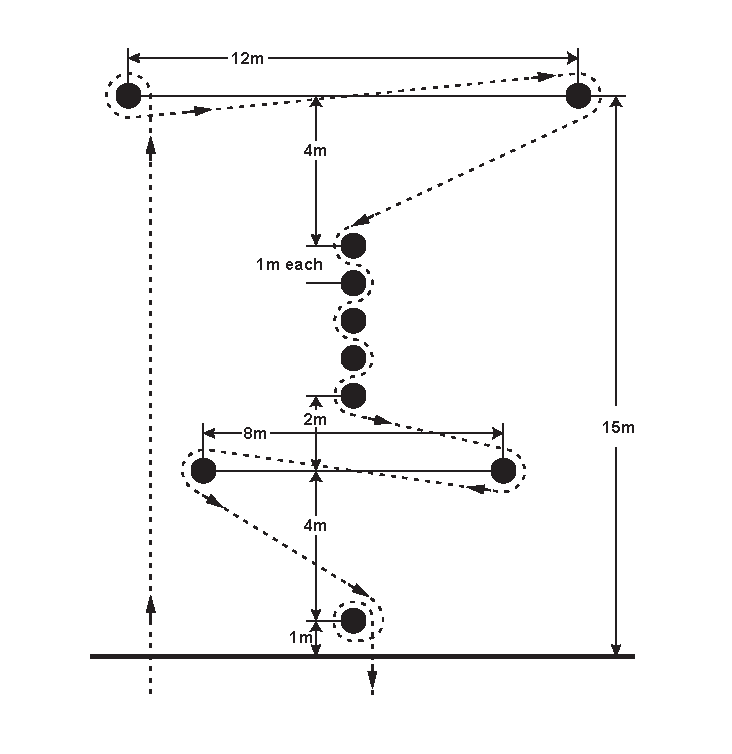
\includegraphics{iuf_slalom}
\end{center}
\vspace{-20pt}
\caption{IUF Slalom Course \label{fig:iuf_slalom}}
\vspace{-10pt}
\end{figure}
Pictured here is the IUF Slalom, in which you must ride around 10 cones in the correct pattern.
Arrows marked on the ground should indicate the direction of the turns for riders unfamiliar with the course.
The rider has to start directly behind the Start line.
The Starter gives the opening, and then the competitor has to start during the next 3 seconds.
The timer is started when any defined point of the tire (for example the part that crosses a low light beam) crosses the start line, and stops when a similar point of the tire crosses the finish line.
If the rider has not yet started after 3 seconds, the timer will start counting anyway.
The rider is not disqualified for this.
Time measurement at start and finish line must be identical to insure accurate time measurement.
It must be secured that riders do not gain momentum before crossing the start line (no flying starts).
Remounting is not allowed.
Cones may be hit, but not knocked over.
The course must be followed correctly, including the direction of turns.
The last cone must be completely circled before the rider's time is taken at the finish line.
Riders who go the wrong way around a cone can go back and make the turn the correct way with the clock still running.
The cones used are plastic traffic cones.
For official competition, cones must be between 45 and 60 cm tall, with bases no more than 30 cm square.
The course must be set up accurately.
The proper positions of the cones should be marked on the ground for a cone to be replaced quickly after it has been knocked over.
Riders get two attempts.

\subsection{Track Coasting}
An event to determine which rider coasts the furthest distance.
There is a 30 meter speed-up distance.
Riders' coasting distances are measured from a `starting line' with a 5 meter minimum, which will be marked by a `qualifying line.'
If the rider does not cross the qualifying line it will count as a failed attempt.
The farthest distance from the line wins.
The distance is measured to the rearmost part of the rider that touches the ground when dismounting, or to the tire contact point where the rider stops coasting.
Remounting is not allowed.
Riders get two attempts.
If a rider crosses the coasting line (tire contact point) not in coasting position, he or she is disqualified in that attempt.
The event should be held on a track or other very level, smooth surface that is as clean as possible. The track may be straight or curved.
Ample time must be allowed for all competitors to make some practice runs on the course before the official start.
Crank arm rules do not apply.
Wind must be at a minimum for records to be set and broken.

\subsection{Track Gliding}

In Gliding, the balance has to be kept all the time by the braking action between one or both feet and the top of the tire.
If, for example, the foot loses contact with the tire due to small bumps, the contact must be restored immediately.
It is held on a track with the same rules as Track Coasting (see above), with the addition that the riding surface must be dry.

\subsection{Downhill Gliding}
In Gliding, the balance has to be kept all the time by the braking action between one or both feet and the top of the tire.
If, for example, the foot loses contact with the tire due to small bumps, the contact must be restored immediately.
A downhill race for speed.
Riders start from a standstill, or speed up to the `starting line.'
Riders are timed over a measured distance to the finish line.
Dismounts before the finish line disqualify the rider in that attempt.
Helmets are mandatory.

\subsection{Slow Balance Forward}

In Slow Balance Forward, the rider rides a distance of 10 meters in a continuous forward motion as slowly as possible without stopping, going backward, hopping or twisting more than 45 degrees to either side.
Any age group with riders of 11 years or older must use a board of 15 cm wide.
Any age group with no riders of 11 years or older must use a board of 30 cm wide at Unicon; in other conventions the host may choose to use either a 15 cm wide board or a 30 cm wide board for this age group.
Tires may overlap the edges of the board, but if the tire contacts the ground next to the board, that would be the end of that attempt.
There are no crank arm length or wheel size restrictions for this event.

Riders must wear shoes.
No other safety gear is required.

\subsubsection{Timing}
The position of the unicycle during Slow Balance is defined by the tire contact point.
In Slow Balance, the rider starts behind the starting line.
On command by the starter, the rider has 10 seconds to start forward motion and let go off the starting post.
The timer starts recording time when the tire contact point crosses the starting line.
At this moment, the rider may not be in contact with the starting post anymore.
Timers must watch the hands and the feet/wheel at the same time at that moment.
The time stops when the tire contact point crosses the finish line.

\subsubsection{Optional Penalty Rules}
At any bigger conventions where there is a large pool of judges (such as Unicon) it is recommended that the host uses a system wherein the judges may give penalties to riders who seem to make ``micro-errors'' or if the judges are in doubt whether an error was made.
Examples of micro-errors are twisting about 46 or 48 degrees, or vibrations of the wheel.
Each penalty subtracts one second from the ridden time.
Riders are still disqualified for clear errors, such as riding off the board, dismounting or twisting 90 degrees.
Using these penalty rules is especially discouraged for possible errors for which a reliable objective detection system is being used.

\subsubsection{Age Group and Final Rounds}
Age Group and Final rounds are always required.

\textbf{Age Group Round:}
\begin{itemize}
\item All riders must participate in the Age Groups.
Riders get two attempts.
\item The best 8 female and the best 8 male riders qualify for the finals.
\item For Unicon a minimum of 20 seconds is required to achieve a valid result.
For any age group with no riders of 11 years or older the minimum time is 15 seconds.
Riders who don't reach this threshold are automatically disqualified.
If your net time after penalties brings you below the minimum time, you are also disqualified.
For other competitions than Unicon, the host may adjust the threshold to a lower time or have no threshold at all.
\end{itemize}

\textbf{Final Round:}
\begin{itemize}
\item The Judging team for the Finals must consist of a single group of people that watch every rider, or (insofar available) an accurate and reliable technical means to check adherence to the rules.
\item Riders get two attempts.
\item The champion is the rider who performs the best result in the final round.
\end{itemize}

\subsection{Slow Balance Backward}
This is the same as Slow Balance Backward, with the following differences \textit {in italic}:
\begin{itemize}
\item Riders ride \textit{backward}.
\item It is an error to ride \textit{forward}.
\item For Unicon a minimum of \textit{15 seconds} is required to achieve a valid result.
For any age group with no riders of 11 years or older the minimum time is \textit{10 seconds}.
\item Any age group with riders of 11 years or older must use a board of \textit{30 cm} wide.
Any age group with no riders of 11 years or older must use a board of \textit{60 cm} wide at Unicon; in other conventions the host may choose to use either a \textit{30 cm} wide board or a \textit{60 cm} wide board for this age group.
\end{itemize}

\subsection{Stillstand}
Stillstand is a competition in which the rider attempts to balance as long as possible.
The rider cannot hop or turn the tire more than 45 degrees, and must remain on a 25 cm long, 10 cm wide, and 3 cm tall block of wood.
The competition should take place indoors on a level surface
The only required safety gear is shoes.

Each participant has 2 attempts that can be done at any time during the time window set by the host.
The host can decide to add to each of the 2 attempts a window up to 20 seconds, in which the competitor can start the number of tries needed.

The starting post is placed anywhere the participant prefers.
Time starts running when the competitor lets go of the starting post.
After time starts running, the starting post will be taken away.
Time stops at the moment when the participant rides off the board, dismounts, starts hopping or turns the tire more than 45 degrees.

There are no finals for the Stillstand competition.
The overall results will be determined by the best results for males and females respectively.
